\chapter{Introduction}

\label{chapter:intro}

Micro unmanned aerial vehicles (MAVs) recently saw a rise in usage across various fields. Drones are already wide used in cinematography \cite{Mademlis2020}, advertising \cite{Ullah2021} and in farming \cite{Kim2019}. 
City emergency departments use UAVs  - firefighters can use them to see and evaluate the situation from the sky, localize the source of fire and put it out \cite{Pritzl2021}. 
They are also quite popular in the military industry.

The inspiration for this project was taken from DJI obstacle avoidance technology introduced with the release of the DJI Mavic 3 drone\footnote{\href{https://www.dji.com/cz/mavic-3}{DJI Mavic 3}}. 
Even though the idea is old, neither DJI, MRS, nor other research groups have a well-developed visual obstacle avoidance system. The best, for now, can be the Skydio system \footnotetext{\href{https://www.skydio.com/skydio-autonomy}{Skydio autonomy}}. 
This direction is very perspective for researchers. Many drones available for sale are costly, and even well-trained pilots are afraid of crashing. 
At the same time, autonomous drones are more predictable than manned, behave according to algorithms, and react much faster, but only if they have a well-designed system running onboard, so obstacle avoidance for autonomous MAVs will be both more challenging and more critical task in future trends.

\section{Related Works}
There are several obstacle avoidance sensors used by various MAVs: stereo vision \cite{Ruf2018}, depth cameras (as Intel RealSense), monocular vision \cite{Mejias2010}, lidar (2d or 3d) \cite{Ramasamy2016}, sonar (ultrasonic), time of flight sensors, also combinations of them can be used. 
In \cite{Rambabu2015} the sensor fusion of ultrasonic and infrared sensors is presented.

Each of them has its pros and cons. 
3D lidars are more expensive than other sensors, but their efficiency is one of the best nowadays; 2d lidars are successfully used for ground vehicles, but they are not so suitable for most tasks for MAVs because a car can be modelled as a 2DoF system, while MAVs always have 6DoF. 
Depth cameras are more expensive than simple cameras. Ultrasonic and infrared sensors have distance limits and other minor issues ( a.e. sonar can be influenced by noise from the MAVs). 

In most articles stereo pair of two parallel cameras looking in the same direction is used (classical stereo pair) \cite{Yu2018, Lin2021, Xiao2019}, deep learning approaches \cite{Back2020, FragaLamas2019, Park2020, Roghair2021} and Convolutional Neural Networks \cite{Yu2013, Ma2020}. 
The real-time multi-camera feedback control system is introduced in \cite{He2021}, but this solution does not imply one drone, only multi-drone systems.

Real-time simultaneous localization and mapping (SLAM) systems can also be used for obstacle avoidance \cite{Moreno2014}. 
These problems are pretty closely related. 
SLAM keeps track of an object's position while constructing and updating a map of an unknown environment; obstacle avoidance is a problem of detecting and avoiding the nearest obstacles in an unknown environment to keep drones safe.
So both problems are related to making a 3D map of an unknown environment, but for obstacle avoidance, the precision of distance measurements to the nearest objects is much more critical.

Structure from Motion (SfM) is another possible algorithm that can be used to implement a system for avoiding obstacles. 
SfM is a method of depth map reconstruction from a set of explicit images, so using this approach, dense point clouds can be computed, and obstacles can be detected \cite{Lee2008}. 

\section{Problem definition}
\begin{figure}[h]
    \centering
    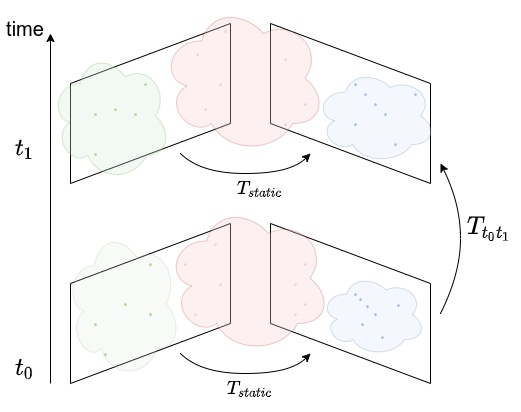
\includegraphics[width=0.7\textwidth]{graphics/general_scheme.png}
    \caption{General system model}
    \label{fig:general}
\end{figure}

This thesis aims to create a visual obstacle avoidance system for MAVs, 3D model, assemble a device, and measure its efficiency. 
The main restrictions for MAV are size and weight: the proposed device should be light and relatively small, and it would be nice to have it cheaper than competitors.

As a basis for software, Robotic operating system (ROS)\footnote{\href{https://www.ros.org/}{ROS home page}} is used, and the MRS UAV system \cite{Baca2021} \footnote{\href{https://github.com/ctu-mrs/mrs_uav_system}{MRS UAV system}} is used as a drone control environment.

The problem solution can be divided into several steps. 
Firstly, it is necessary to make a math model of a device that can solve the problem and describe its behaviour. 
The next step is to make a CAD model of the cameras' holder, print and assemble it, and then calibrate it. 
Then detect features and compute the distance to visible objects in cameras' overlapping zone: as far as a stereo pair is calibrated, the precision depends on a stereo pair calibration, cameras' calibration, key point extractor and matcher.
As a result, provided points and features can be used in an SfM algorithm to correct a relative stereo pair position in time while moving and in a feedback loop inside the MRS system to correct its path planning concerning found obstacles.
